% !TeX root = ../Studienarbeit.tex

\addchap{Anhang}
{\Large
\begin{enumerate}[label=\Alph*.]
	\item Schaltpläne
\end{enumerate}
}
\pagebreak
\section*{A.Schaltpläne}
\begin{figure}[htp]
    \centering
    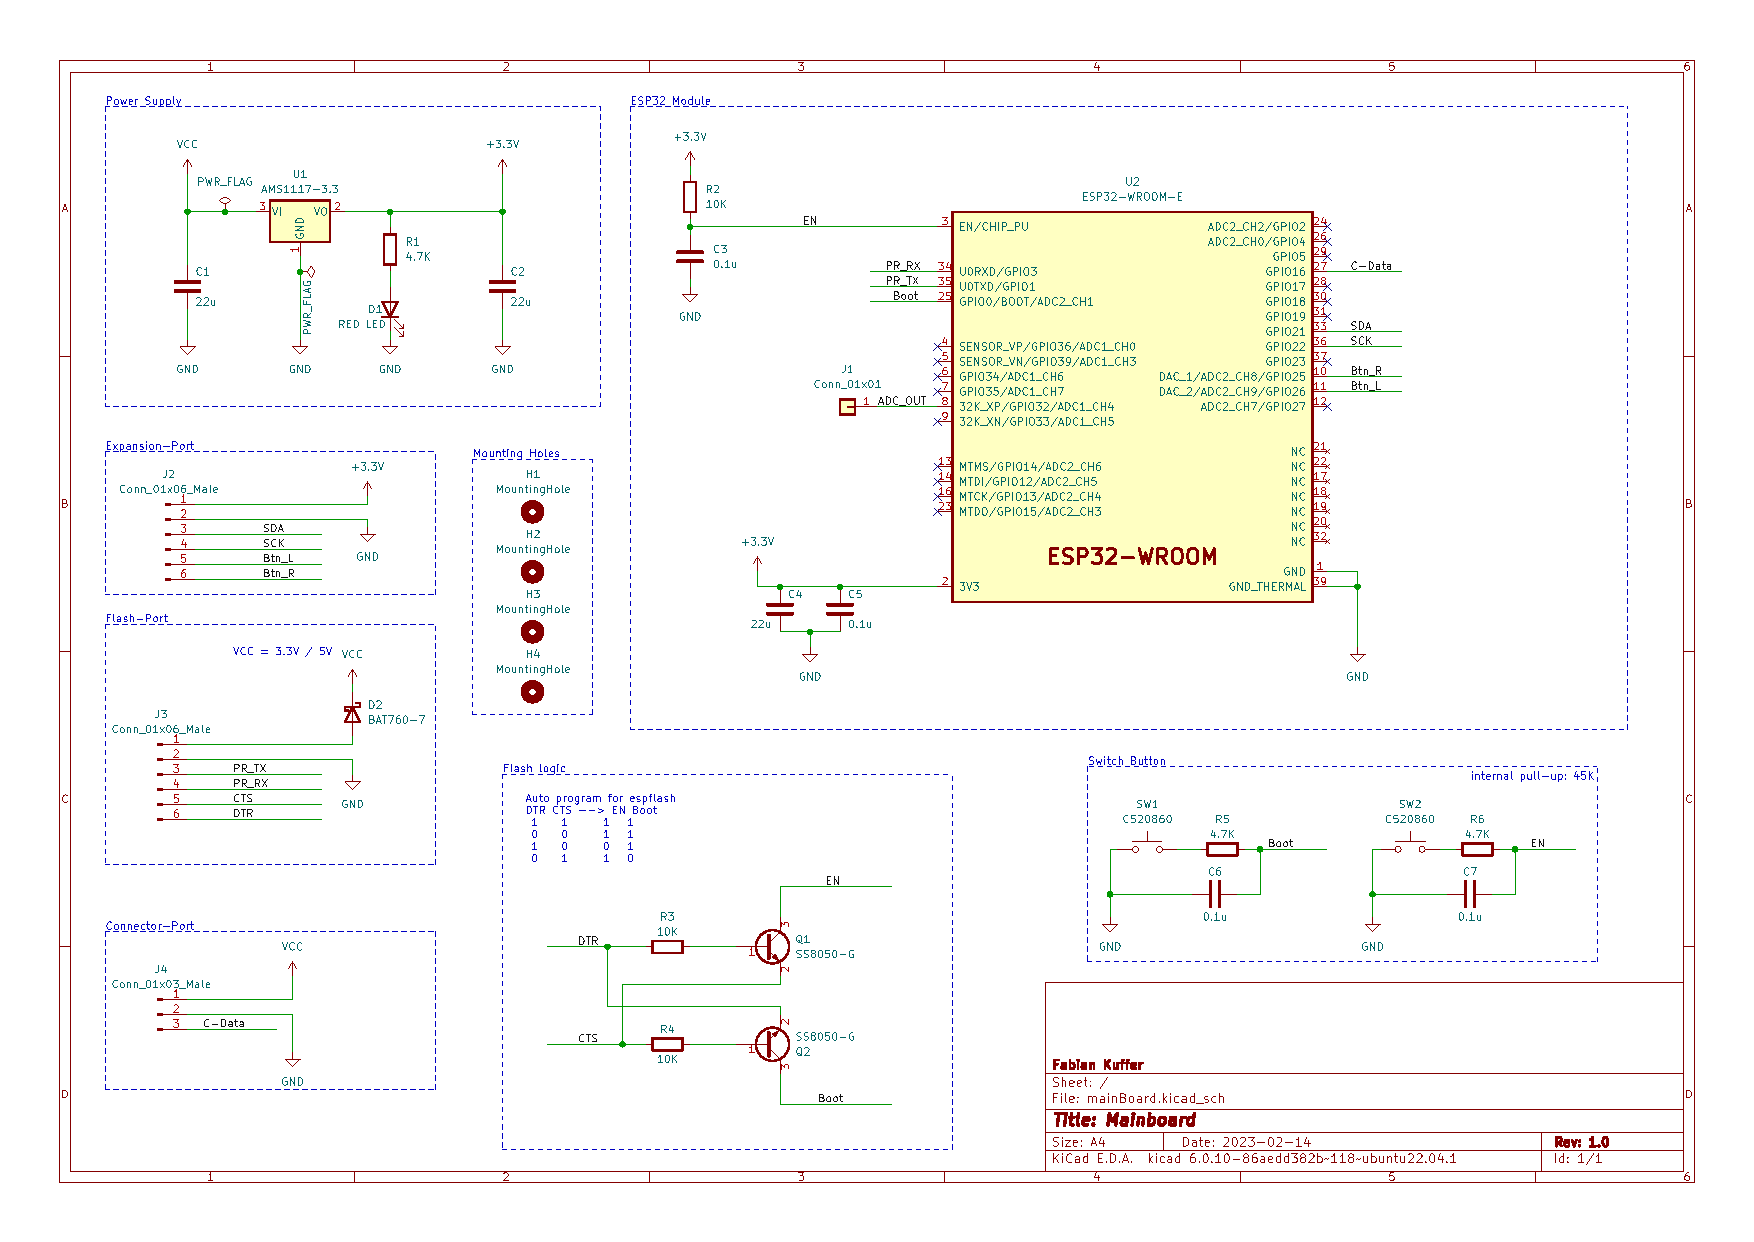
\includegraphics[width=1\textwidth]{../PDFs/mainBoard.pdf}
    \caption{Schaltplan der Hauptplatine}
    \label{fig:mainPCB}
\end{figure}

\begin{figure}[htp]
    \centering
    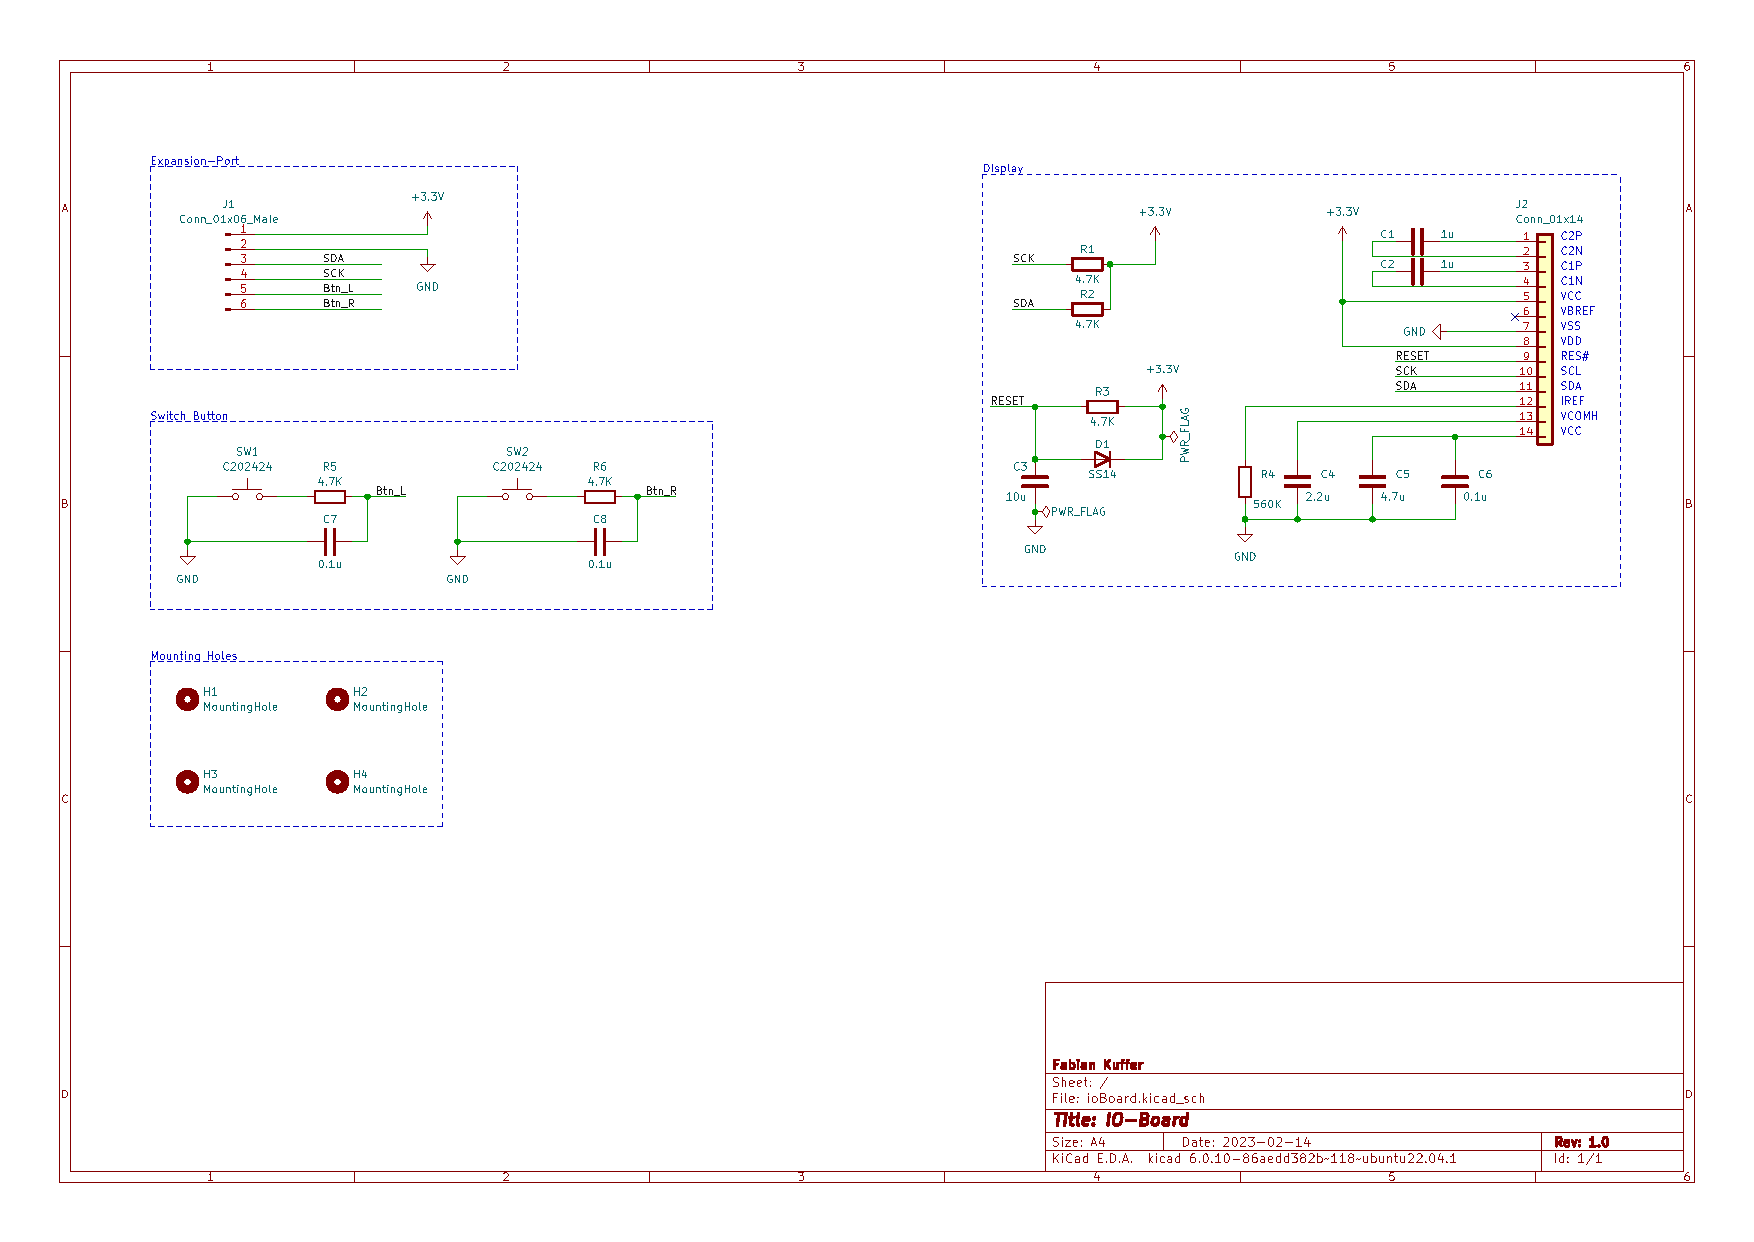
\includegraphics[width=1\textwidth]{../PDFs/ioBoard.pdf}
    \caption{Schaltplan für Ein- und Ausgabekomponenten}
    \label{fig:ioPCB}
\end{figure}

\begin{figure}[htp]
    \centering
    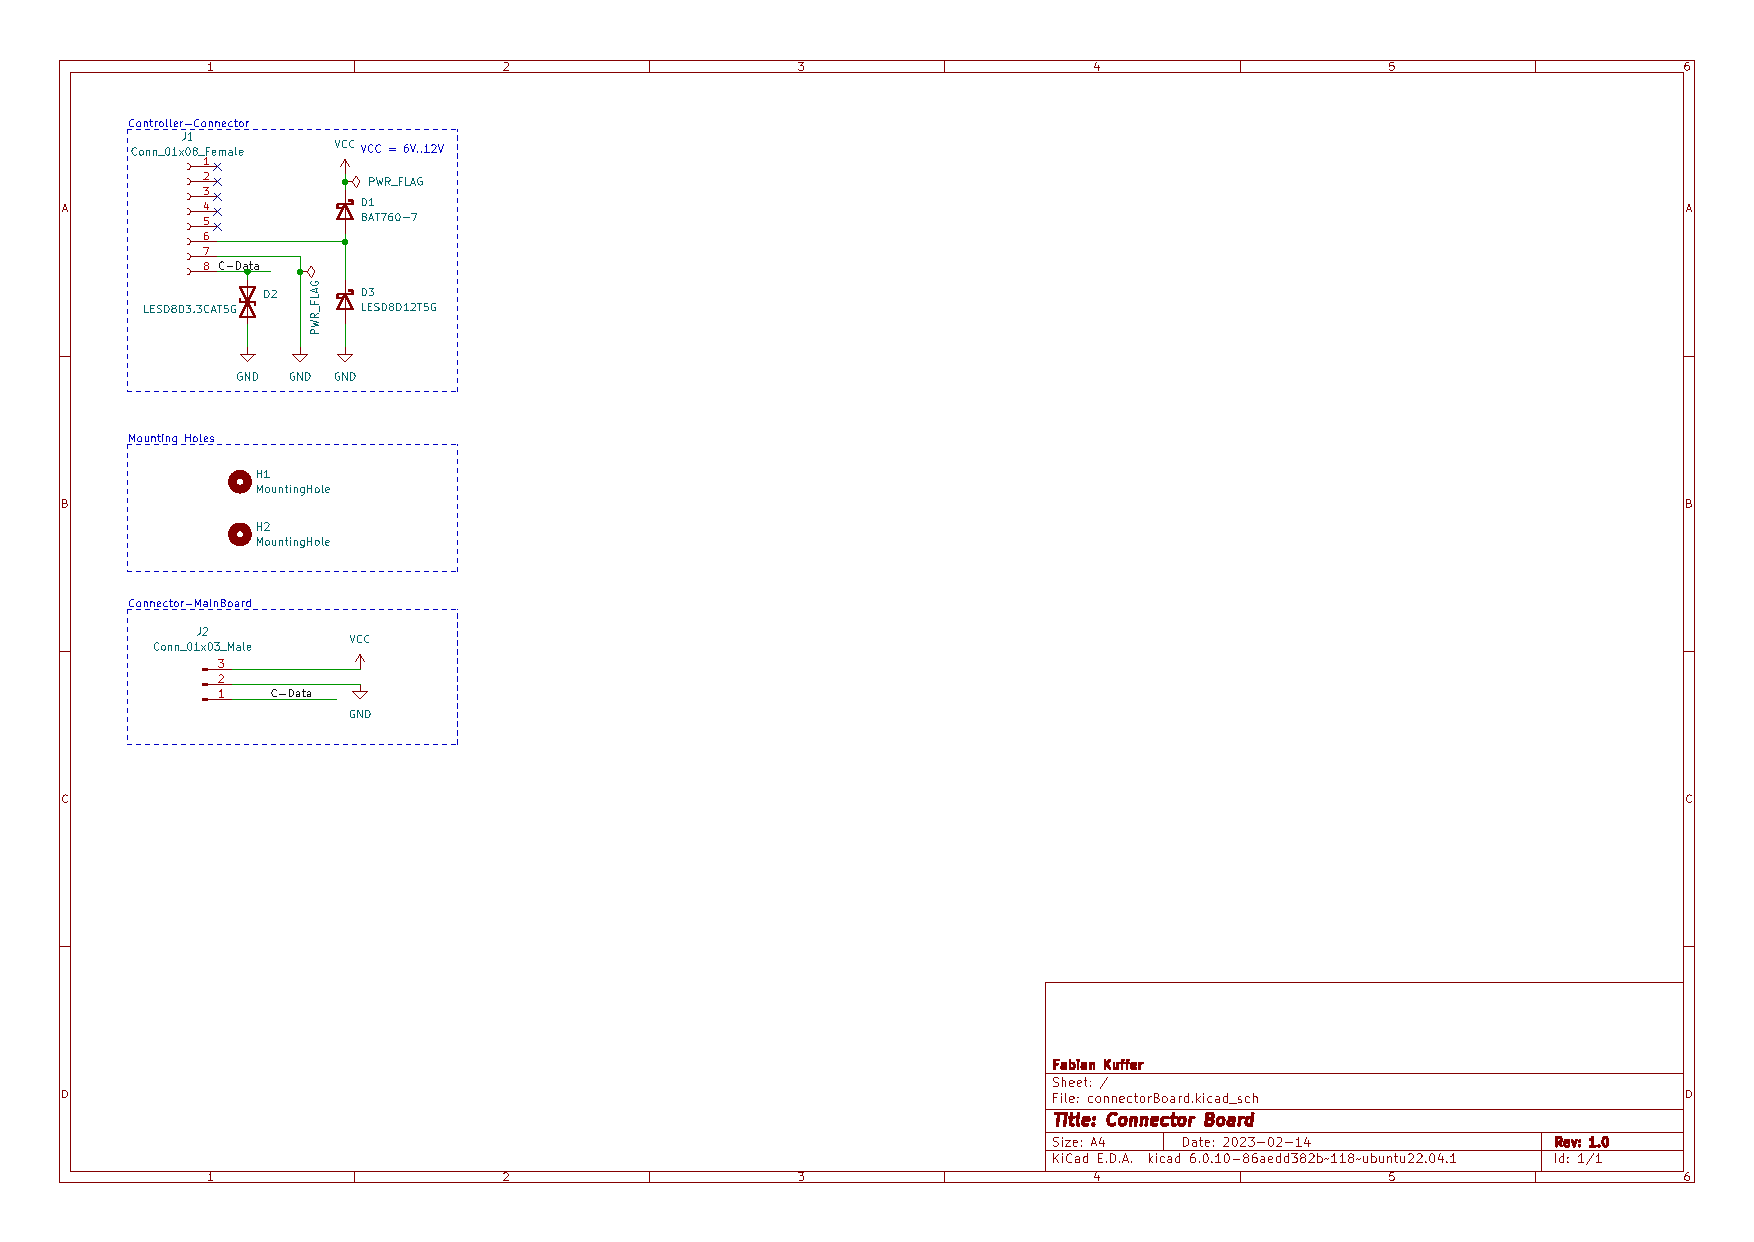
\includegraphics[width=1\textwidth]{../PDFs/connectorBoard.pdf}
    \caption{Schaltplan für die Verbindung zwischen Erweiterungsmodul und Multikopterfernsteuerung}
    \label{fig:connectorPCB}
\end{figure}